% FONTE TEMA https://github.com/matze/mtheme
\documentclass[aspectratio=1610]{beamer}
%\documentclass[aspectratio=1610, handout]{beamer}
\usepackage[utf8]{inputenc}
\usepackage{ragged2e}
\usepackage{xcolor}
\usepackage[italian]{babel}
\usepackage{multirow}
\usepackage{silence}
\WarningFilter{beamer}{}
\WarningFilter{metropolis}{}
\usetheme[progressbar=frametitle,titleformat=smallcaps]{metropolis}
\setbeamertemplate{frame numbering}[fraction]
\setbeamercovered{dynamic}
\definecolor{rosso}{RGB}{255, 0, 0}
\definecolor{giallo}{RGB}{254,212,23}
\hypersetup{colorlinks=true,linkcolor=black,urlcolor=rosso}
\setbeamercolor{palette primary}{fg=black, bg=giallo}
\setbeamercolor{background canvas}{bg=white}
\setbeamercolor{normal text}{fg=black}
\setbeamercolor{progress bar}{fg=rosso}
\setbeamercolor{framesubtitle}{fg=rosso}
\setbeamercolor{normal text .dimmed}{fg=giallo}
\setbeamercolor{block title alerted}{fg=rosso, bg=giallo}
\setbeamerfont{caption}{size=\tiny}
\setbeamerfont{caption name}{size=\tiny}
\setlength{\abovecaptionskip}{0pt}
\makeatletter
\metroset{block=fill}
\setlength{\metropolis@progressinheadfoot@linewidth}{1pt} 
\setlength{\metropolis@progressonsectionpage@linewidth}{1pt}
\setlength{\metropolis@titleseparator@linewidth}{1pt}
\makeatother

\title{GERARCHIE DI GENERALIZZAZIONE}
\subtitle{Ereditarietà}
\date{}
\institute{\textit{
        Fonti:
        \begin{itemize}
            \item[-] \href{https://it.wikipedia.org/wiki/Modello_E-R}{Wikipedia}
        \end{itemize}
    }
}

\begin{document}

\begin{frame}[plain, noframenumbering]
    \titlepage
\end{frame}

\begin{frame}{GERARCHIA DI GENERALIZZAZIONE}
    \begin{alertblock}{DEFINIZIONE}
        \begin{minipage}{0.98\linewidth}
            \justifying
            Una gerarchia di generalizzazione è un legame logico tra un'entità padre E ed alcune entità figlie $E_1, E_2 ... E_n$ dove:
            \begin{itemize}
                \item[-] E è la \textbf{GENERALIZZAZIONE} di $E_1, E_2 ... E_n$
                \item[-] $E_1, E_2 ... E_n$ sono \textbf{SPECIALIZZAZIONI} di E
            \end{itemize}
            tale per cui:
            \begin{itemize}
                \item[-] Ogni istanza di $E_i$ è anche un'istanza di E
                \item[-] Una istanza di E può essere un'istanza di una o più entità $E_i$
            \end{itemize}
        \end{minipage}
    \end{alertblock}
\end{frame}

\begin{frame}{EREDITARIET\'A}
    Le entità figlie ereditano le proprietà (attributi, associazioni, identificatori) dell'entità padre.
    \begin{figure}
        \includegraphics[width=.8\linewidth]{img/ereditarietà.png}
        \caption{{creata con \href{https://app.diagrams.net/}{Diagrams.net}}}
    \end{figure}
\end{frame}

\begin{frame}{GERARCHIE TOTALI O PARZIALI}
    \begin{columns}
        \column{.5\textwidth}
            \begin{alertblock}{DEFINIZIONE}
                \begin{minipage}{0.96\linewidth}
                    \justifying
                    Ogni \textbf{gerarchia di generalizzazione} è o \textbf{totale} o \textbf{parziale}:\\
                    \bigskip
                    \textbf{TOTALE} (t): Ogni istanza dell'entità padre deve fare parte di una delle entità figlie.\\
                    \bigskip
                \end{minipage}
            \end{alertblock}
        \column{.5\textwidth}
            \begin{figure}
        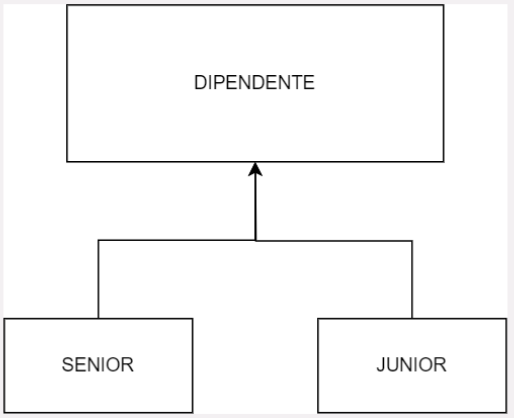
\includegraphics[width=.8\linewidth]{img/totale.png}
        \caption{{creata con \href{https://app.diagrams.net/}{Diagrams.net}}}
            \end{figure}
    \end{columns}
\end{frame}

\begin{frame}{GERARCHIE TOTALI O PARZIALI}
    \begin{columns}
        \column{.5\textwidth}
            \begin{alertblock}{DEFINIZIONE}
                \begin{minipage}{0.96\linewidth}
                    \justifying
                    Ogni \textbf{gerarchia di generalizzazione} è o \textbf{totale} o \textbf{parziale}:\\
                    \bigskip
                    \textbf{PARZIALE} (p): Le istanze dell'entità padre possono far parte di una delle entità figlie.\\
                    \bigskip
                \end{minipage}
            \end{alertblock}
        \column{.5\textwidth}
            \begin{figure}
        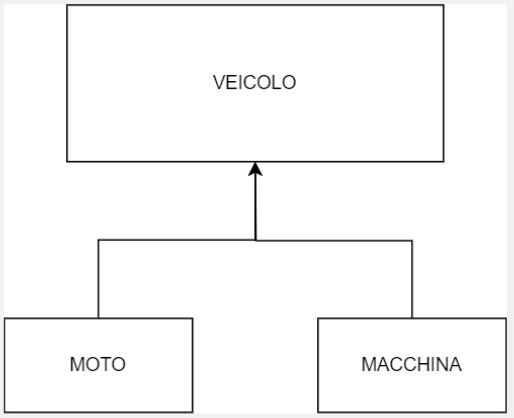
\includegraphics[width=.8\linewidth]{img/parziale.png}
        \caption{{creata con \href{https://app.diagrams.net/}{Diagrams.net}}}
            \end{figure}
    \end{columns}
\end{frame}

\begin{frame}{GERARCHIE ESCLUSIVE O SOVRAPPOSTE}
    \begin{columns}
        \column{.5\textwidth}
            \begin{alertblock}{DEFINIZIONE}
                \begin{minipage}{0.96\linewidth}
                    \justifying
                    Ogni \textbf{gerarchia di generalizzazione} è o \textbf{esclusiva} o \textbf{sovrapposta}:\\
                    \bigskip
                    \textbf{ESCLUSIVA} (e): Ogni istanza dell'entità padre \textbf{non può} far parte di più di una delle entità figlie.\\
                    \bigskip
                \end{minipage}
            \end{alertblock}
        \column{.5\textwidth}
            \begin{figure}
        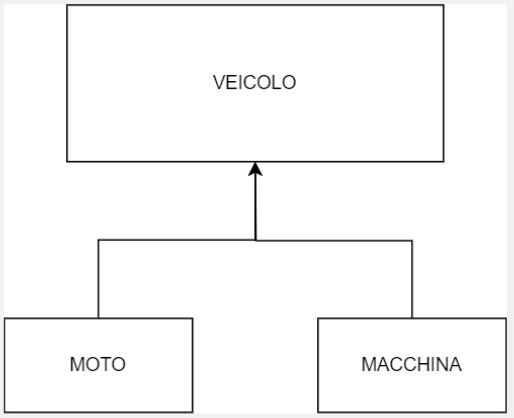
\includegraphics[width=.8\linewidth]{img/parziale.png}
        \caption{{creata con \href{https://app.diagrams.net/}{Diagrams.net}}}
            \end{figure}
    \end{columns}
\end{frame}

\begin{frame}{GERARCHIE ESCLUSIVE O SOVRAPPOSTE}
    \begin{columns}
        \column{.5\textwidth}
            \begin{alertblock}{DEFINIZIONE}
                \begin{minipage}{0.96\linewidth}
                    \justifying
                    Ogni \textbf{gerarchia di generalizzazione} è o \textbf{esclusiva} o \textbf{sovrapposta}:\\
                    \bigskip
                    \textbf{SOVRAPPOSTA} (e): Ogni istanza dell'entità padre \textbf{può} far parte di più di una delle entità figlie.\\
                    \bigskip
                \end{minipage}
            \end{alertblock}
        \column{.5\textwidth}
            \begin{figure}
        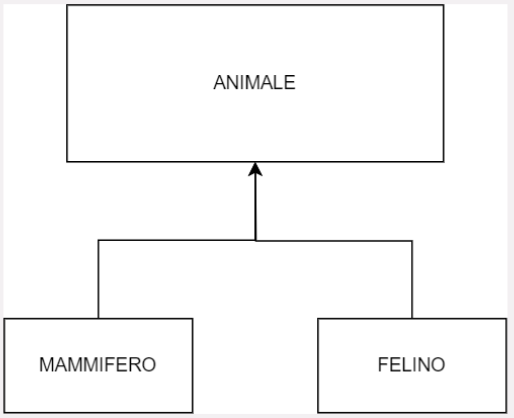
\includegraphics[width=.8\linewidth]{img/sovrapposta.png}
        \caption{{creata con \href{https://app.diagrams.net/}{Diagrams.net}}}
            \end{figure}
    \end{columns}
\end{frame}

\begin{frame}{GERARCHIE DI GENERALIZZAZIONE}
    Esistono quindi quattro tipi di gerarchie di generalizzazione:
    \pause
    \begin{itemize}
        \item \textbf{(t,e)}: GERARCHIA TOTALE ED ESCLUSIVA;
        \pause
        \item \textbf{(t,s)}: GERARCHIA TOTALE E SOVRAPPOSTA;
        \pause
        \item \textbf{(p,e)}: GERARCHIA PARZIALE ED ESCLUSIVA;
        \pause
        \item \textbf{(p,s)}: GERARCHIA PARZIALE E SOVRAPPOSTA.
    \end{itemize}
\end{frame}

\end{document}